% -- \include{b2cincl.tex}
% ======================================================================
\subsection{Inclusive CKM-favored decays}
\label{slbdecays_b2cincl}
% -------------------------------------------

\subsubsection{Global analysis of $\bar B\to X_c\ell^-\bar\nu_\ell$}

The semileptonic width $\Gamma(\bar B\to X_c\ell^-\bar\nu_\ell)$ has
been calculated in the framework of the Operator Product
Expansion. The result is a double-expansion in $\Lambda_{\rm QCD}/m_b$
and $\alpha_s$, which depends on a number of non-perturbative
parameters. These parameters can be measured using other observables
in $\bar B\to X_c\ell^-\bar\nu_\ell$ decays, such as the moments of
the lepton energy and the hadronic mass spectrum.

Two independent sets of theoretical expressions, referred to as
kinetic~\cite{Benson:2003kp,Gambino:2004qm,Gambino:2011cq} and 1S
schemes~\cite{Bauer:2004ve} are available for this kind of
analysis. The non-perturbative parameters in the kinetic scheme
are: the quark masses $m_b$ and $m_c$, $\mu^2_\pi$ and
$\mu^2_G$ at $O(1/m^2_b)$, and $\rho^3_D$ and $\rho^3_{LS}$ at
$O(1/m^3_b)$. In the 1S scheme, the parameters are: $m_b$, $\lambda_1$
at $O(1/m^2_b)$, and $\rho_1$, $\tau_1$, $\tau_2$ and $\tau_3$ at
$O(1/m^3_b)$. Note that due to the different definitions, the results
for the quark masses cannot be compared directly between the two
schemes.

Our analysis uses all available measurements of moments in $\bar B\to
X_c\ell^-\bar\nu_\ell$, excluding only points with too high
correlation to avoid numerical issues. The list of included
measurements is given in
Table~\ref{tab:gf_input}. The only external input is the average
lifetime~$\tau_B$ of neutral and charged $B$~mesons, taken to be
$(1.579\pm 0.005)$~ps (Sect.~\ref{sec:life_mix}).
\begin{table}[!htb]
\caption{Experimental inputs used in the global analysis of $\bar B\to
  X_c\ell^-\bar\nu_\ell$. $n$ is the order of the moment, $c$ is the
  threshold value in GeV. In total, there are 23 measurements from
  \babar, 15 measurements from Belle and 12 from other
  experiments.} \label{tab:gf_input}
\begin{center}
\begin{tabular}{|l|l|l|}
  \hline
  Experiment
  & Hadron moments $\langle M^n_X\rangle$
  & Lepton moments $\langle E^n_\ell\rangle$\\
  \hline \hline
  \babar & $n=2$, $c=0.9,1.1,1.3,1.5$ & $n=0$, $c=0.6,1.2,1.5$\\
  & $n=4$, $c=0.8,1.0,1.2,1.4$ & $n=1$, $c=0.6,0.8,1.0,1.2,1.5$\\
  & $n=6$, $c=0.9,1.3$~\cite{Aubert:2009qda} & $n=2$, $c=0.6,1.0,1.5$\\
  & & $n=3$, $c=0.8,1.2$~\cite{Aubert:2009qda,Aubert:2004td}\\
  \hline
  Belle & $n=2$, $c=0.7,1.1,1.3,1.5$ & $n=0$, $c=0.6,1.4$\\
  & $n=4$, $c=0.7,0.9,1.3$~\cite{Schwanda:2006nf} & $n=1$,
  $c=1.0,1.4$\\
  & & $n=2$, $c=0.6,1.4$\\
  & & $n=3$, $c=0.8,1.2$~\cite{Urquijo:2006wd}\\
  \hline
  CDF & $n=2$, $c=0.7$ & \\
  & $n=4$, $c=0.7$~\cite{Acosta:2005qh} & \\
  \hline
  CLEO & $n=2$, $c=1.0,1.5$ & \\
  & $n=4$, $c=1.0,1.5$~\cite{Csorna:2004kp} & \\
  \hline
  DELPHI & $n=2$, $c=0.0$ & $n=1$, $c=0.0$ \\
  & $n=4$, $c=0.0$ & $n=2$, $c=0.0$ \\
  & $n=6$, $c=0.0$~\cite{Abdallah:2005cx} & $n=3$,
  $c=0.0$~\cite{Abdallah:2005cx}\\
  \hline
\end{tabular}
\end{center}
\end{table}

Both in the kinetic and 1S scheme, the moments in $\bar B\to
X_c\ell^-\bar\nu_\ell$ are not sufficient to constrain the $b$-quark
mass precisely. In the kinetic scheme analysis we fix the $c$-quark
mass (defined in the $\overline{\rm MS}$ scheme) to the value of
Ref.~\cite{Chetyrkin:2009fv},
\begin{equation}
  m_c^{\overline{\rm MS}}(3~{\rm GeV})=(0.986\pm 0.013)~{\rm GeV}~.
\end{equation}
In the 1S~scheme analysis, the $b$-quark mass is constrained with
measurements of the photon energy moments in $B\to
X_s\gamma$~\cite{Aubert:2005cua,Aubert:2006gg,Limosani:2009qg,Chen:2001fja}.

\subsubsection{Analysis in the kinetic scheme}
\label{globalfitsKinetic}

The fit relies on the calculations of the spectral moments in $\bar
B\to X_c\ell^-\bar\nu_\ell$~decays described in
Ref.~\cite{Gambino:2011cq} and closely follows the procedure of
Ref.~\cite{Gambino:2013rza}. The analysis determines $\vcb$ and the 6
non-perturbative parameters mentioned above.

The result in terms of the main parameters is
\begin{eqnarray}
  \vcb & = & (42.46\pm 0.88)\times 10^{-3}~, \\
  m_b^{\rm kin} & = & 4.541\pm 0.023~{\rm GeV}~, \\
  \mu^2_\pi & = & 0.414\pm 0.078~{\rm GeV^2}~,
\end{eqnarray}
with a $\chi^2$ of 14.6 for $50-7$ degrees of freedom. The detailed
result and the matrix of the correlation coefficients is given in
Table~\ref{tab:gf_res_mc_kin}. The fit to the lepton energy and
hadronic mass moments is shown in Figs.~\ref{fig:gf_res_kin_el} and
\ref{fig:gf_res_kin_mx}, respectively.
\begin{table}[!htb]
\caption{Fit result in the kinetic scheme, using a precise $c$-quark
  mass constraint. The error matrix of the fit contains
  experimental and theoretical contributions. In the lower part of the
  table, the correlation matrix of the parameters is
  given.} \label{tab:gf_res_mc_kin}
\begin{center}
\resizebox{0.99\textwidth}{!}{
\begin{tabular}{|l|ccccccc|}
  \hline
  & \vcb\ [10$^{-3}$] & $m_b^{\rm kin}$ [GeV] &
  $m_c^{\overline{\rm MS}}$ [GeV] & $\mu^2_\pi$ [GeV$^2$]
  & $\rho^3_D$ [GeV$^3$] & $\mu^2_G$ [GeV$^2$] & $\rho^3_{LS}$ [GeV$^3$]\\
  \hline \hline
  value & 42.46 & \phantom{$-$}4.541 & \phantom{$-$}0.987 &
  \phantom{$-$}0.414 & \phantom{$-$}0.154 & \phantom{$-$}0.340 &
  $-$0.147\\
  error & 0.88 & \phantom{$-$}0.023 &
  \phantom{$-$}0.013 & \phantom{$-$}0.078 & \phantom{$-$}0.045 &
  \phantom{$-$}0.066 & \phantom{$-$}0.098\\
  \hline
  $|V_{cb}|$ & 1.000 & $-$0.466 & $-$0.049 &
  \phantom{$-$}0.344 & \phantom{$-$}0.161 & $-$0.190 &
  \phantom{$-$}0.019\\
  $m_b^{\rm kin}$ & & \phantom{$-$}1.000 & \phantom{$-$}0.506 &
  $-$0.113 & \phantom{$-$}0.219 & \phantom{$-$}0.487 & $-$0.156\\
  $m_c^{\overline{\rm MS}}$ & & & \phantom{$-$}1.000
  & $-$0.018 & \phantom{$-$}0.020 & \phantom{$-$}0.008 & $-$0.002\\
  $\mu^2_\pi$ & & & & \phantom{$-$}1.000 & \phantom{$-$}0.610 &
  \phantom{$-$}0.001 & \phantom{$-$}0.058\\
  $\rho^3_D$ & & & & & \phantom{$-$}1.000 & $-$0.038 & $-$0.126\\
  $\mu^2_G$ & & & & & & \phantom{$-$}1.000 & $-$0.014\\
  $\rho^3_{LS}$ & & & & & & & \phantom{$-$}1.000\\
  \hline
\end{tabular}
}
\end{center}
\end{table}
\begin{figure}
\begin{center}
  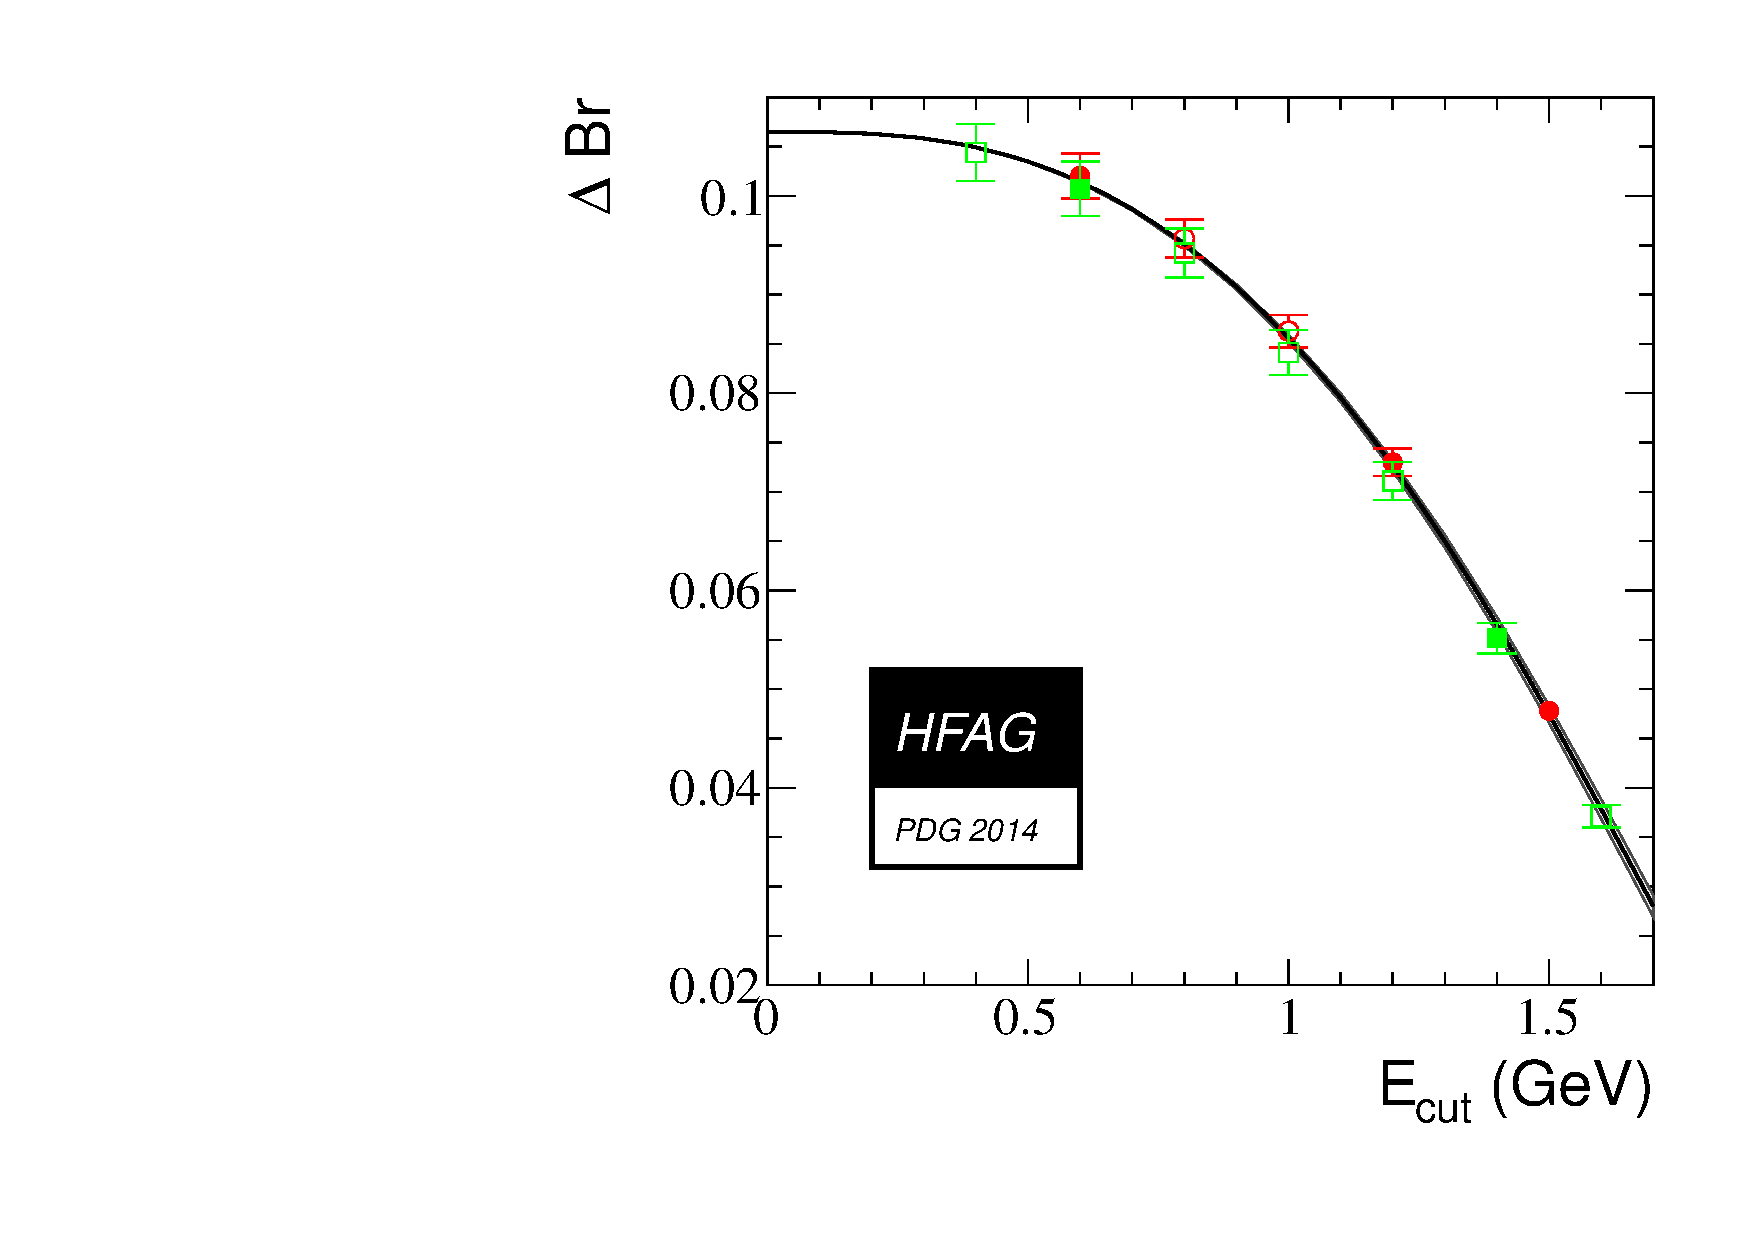
\includegraphics[width=7cm]{figures/slb/e0_1.pdf}
  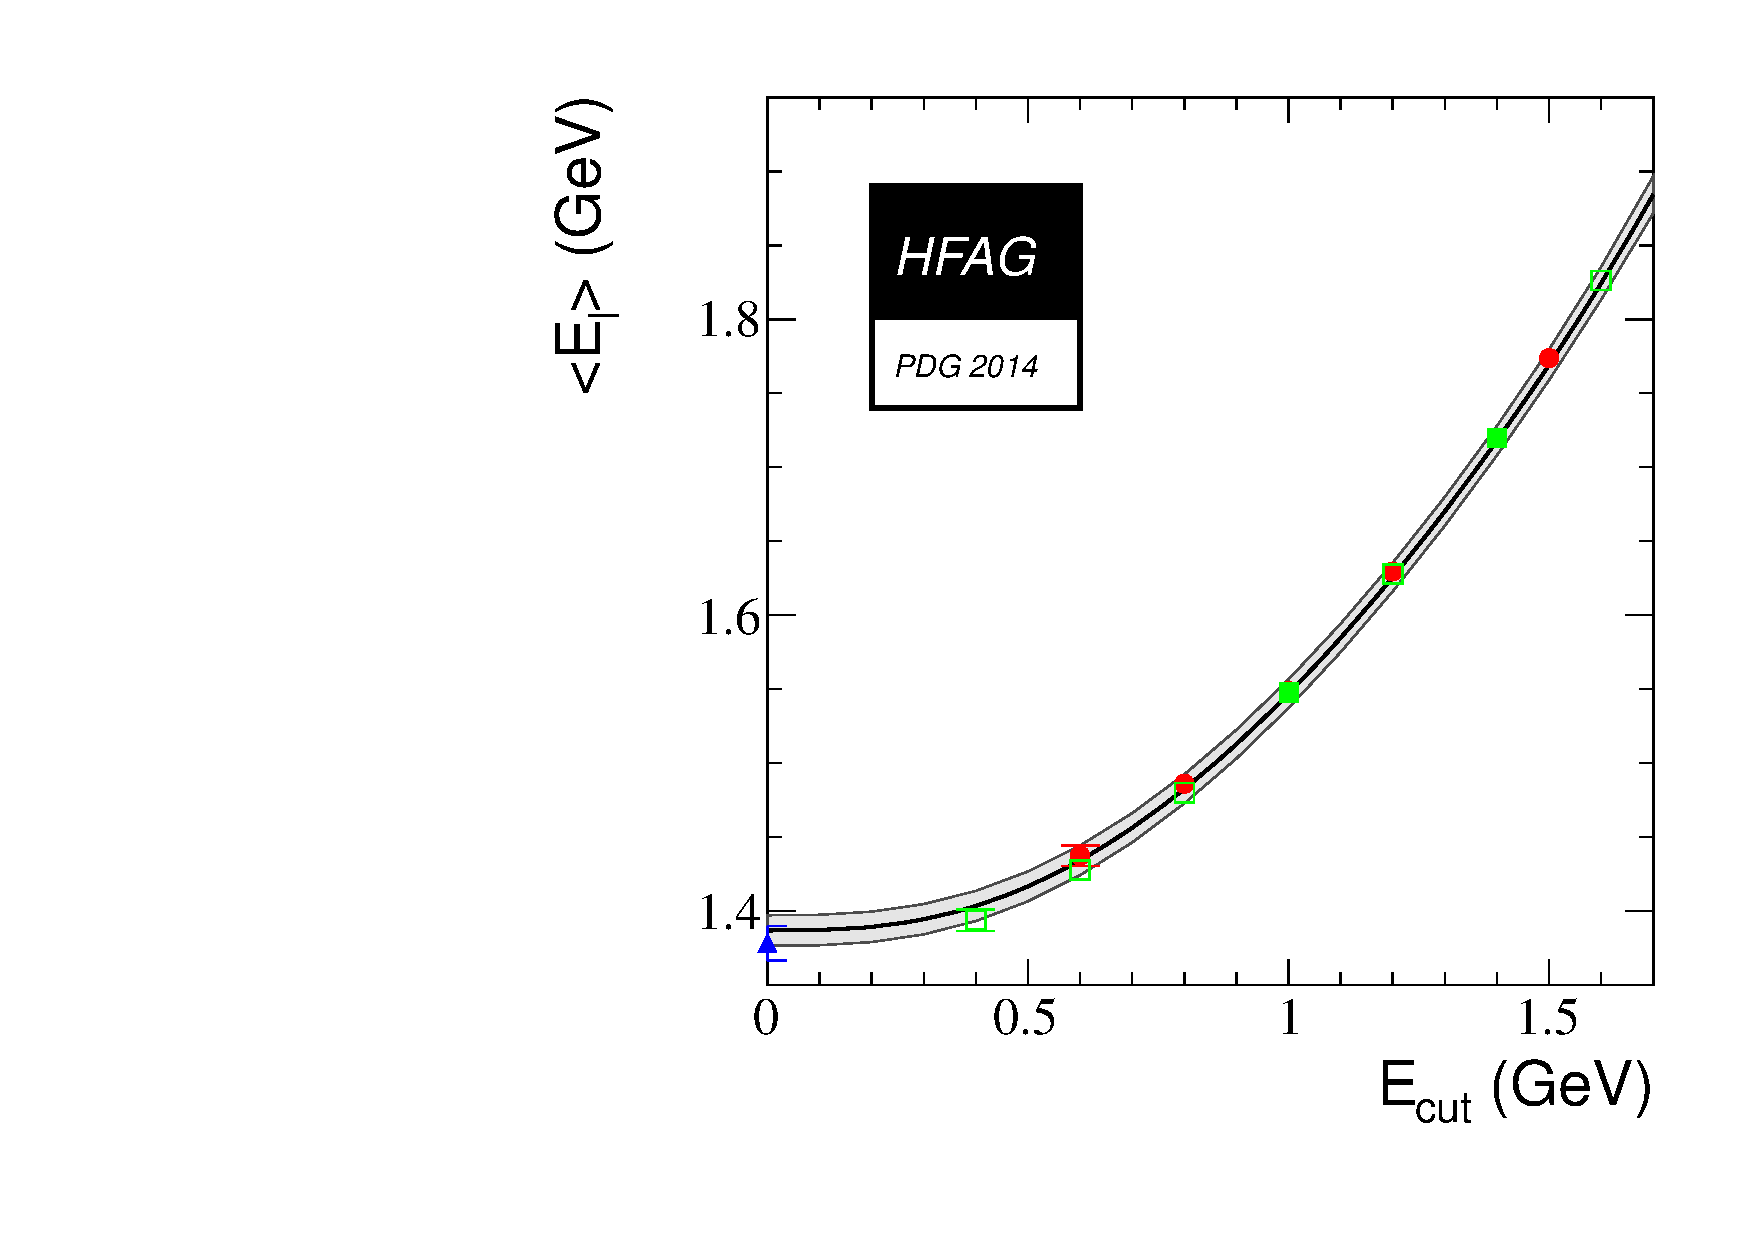
\includegraphics[width=7cm]{figures/slb/e1_1.pdf}\\
  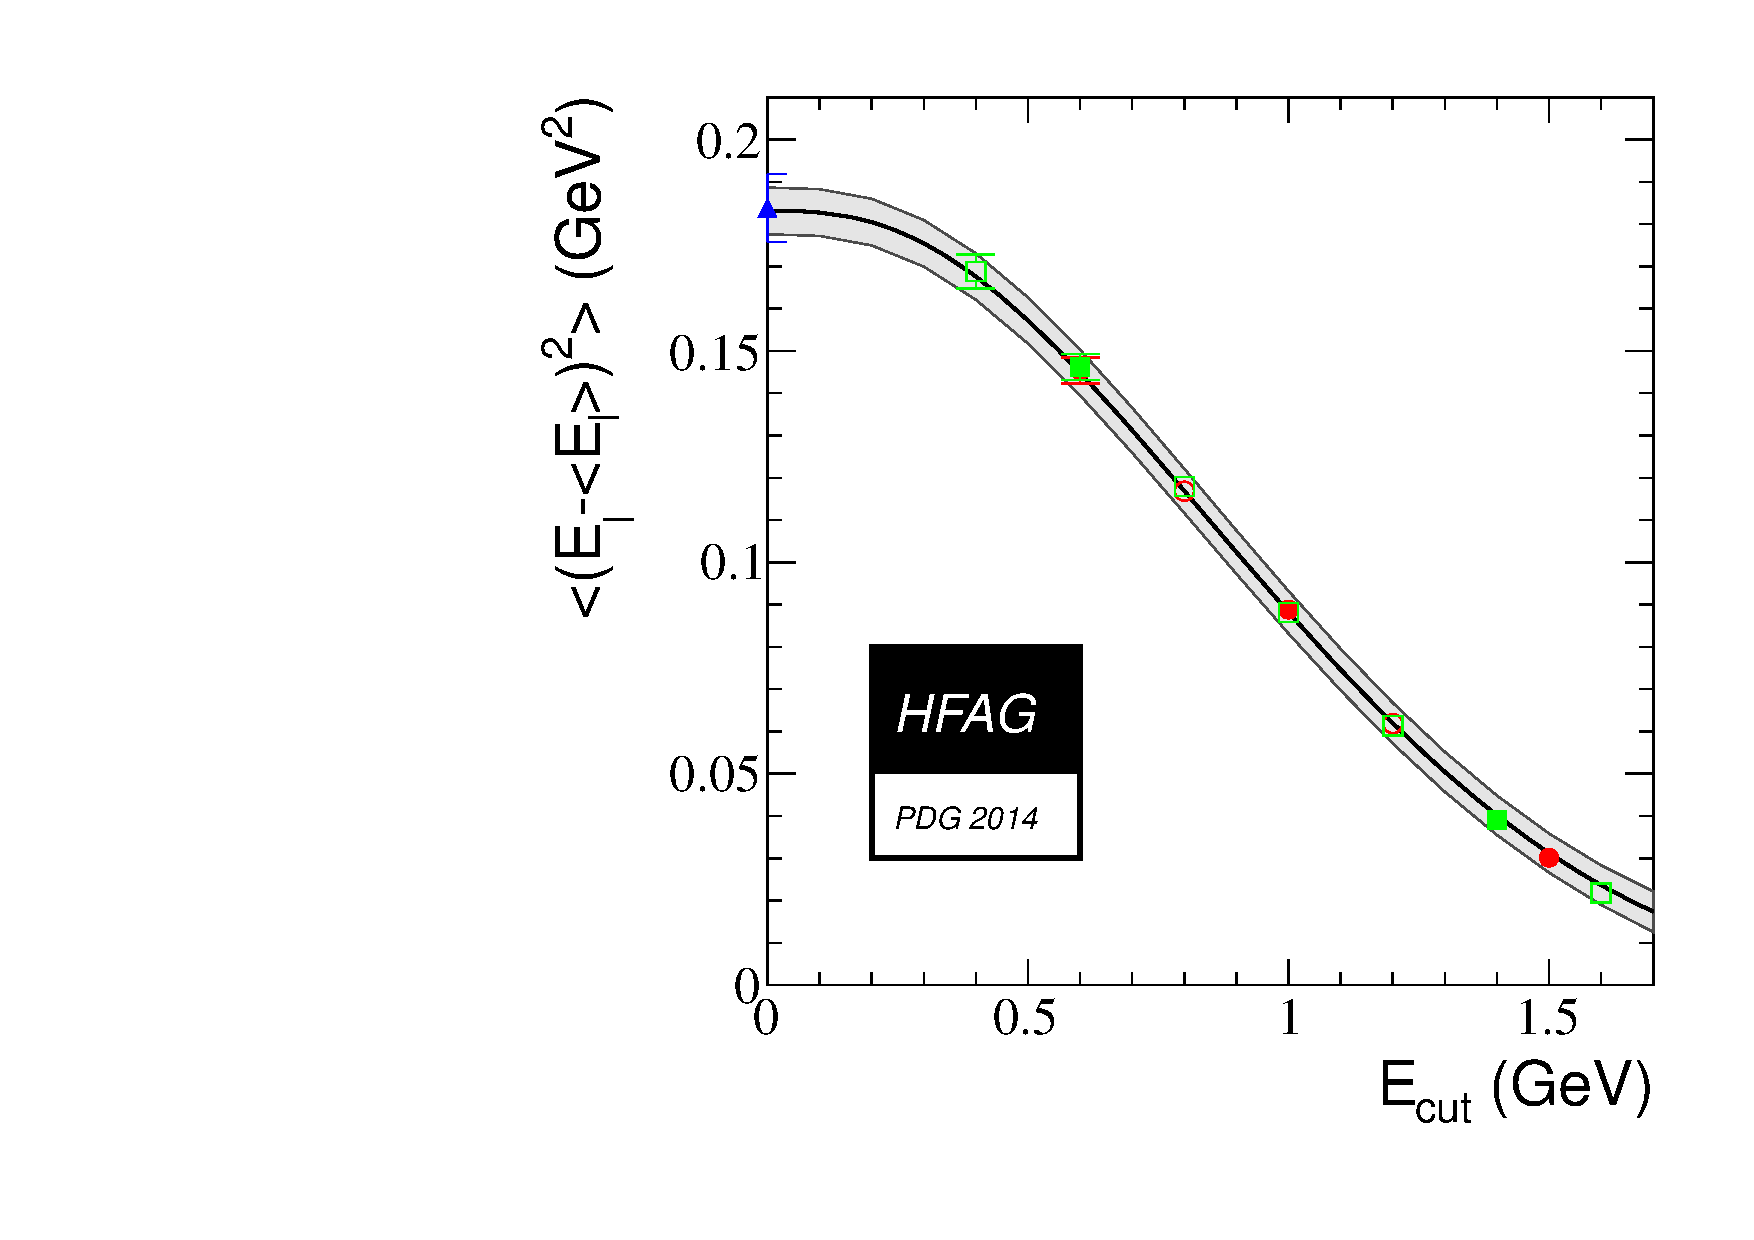
\includegraphics[width=7cm]{figures/slb/e2_1.pdf}
  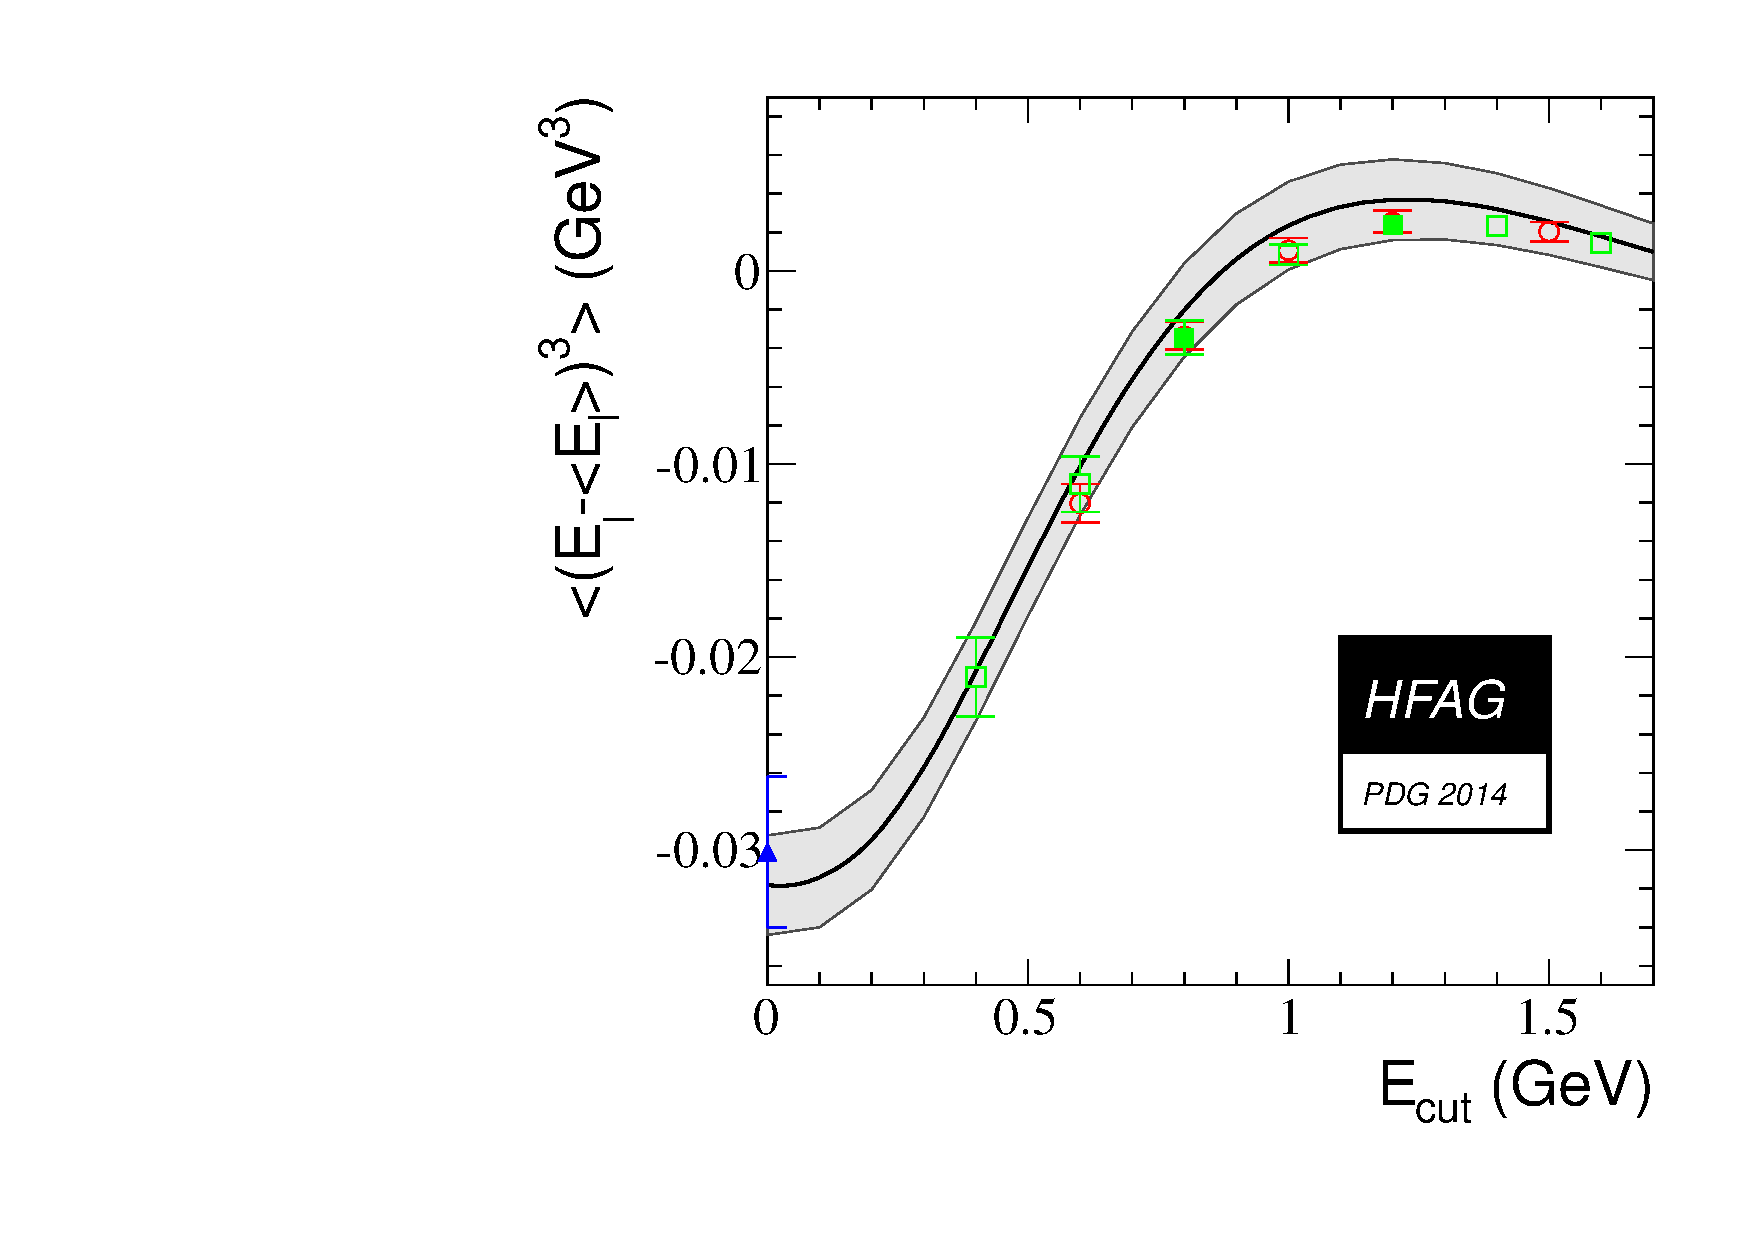
\includegraphics[width=7cm]{figures/slb/e3_1.pdf}
\end{center}
\caption{Fit to the partial semileptonic branching ratios and to the
  lepton energy moments in the kinetic mass scheme. In all plots, the
  grey band is the theory prediction with total theory error. \babar
  data are shown by circles, Belle by squares and other experiments
  (DELPHI, CDF, CLEO) by triangles. Filled symbols mean that the point
  was used in the fit. Open symbols are measurements that were not
  used in the fit.} \label{fig:gf_res_kin_el}
\end{figure}
\begin{figure}
\begin{center}
  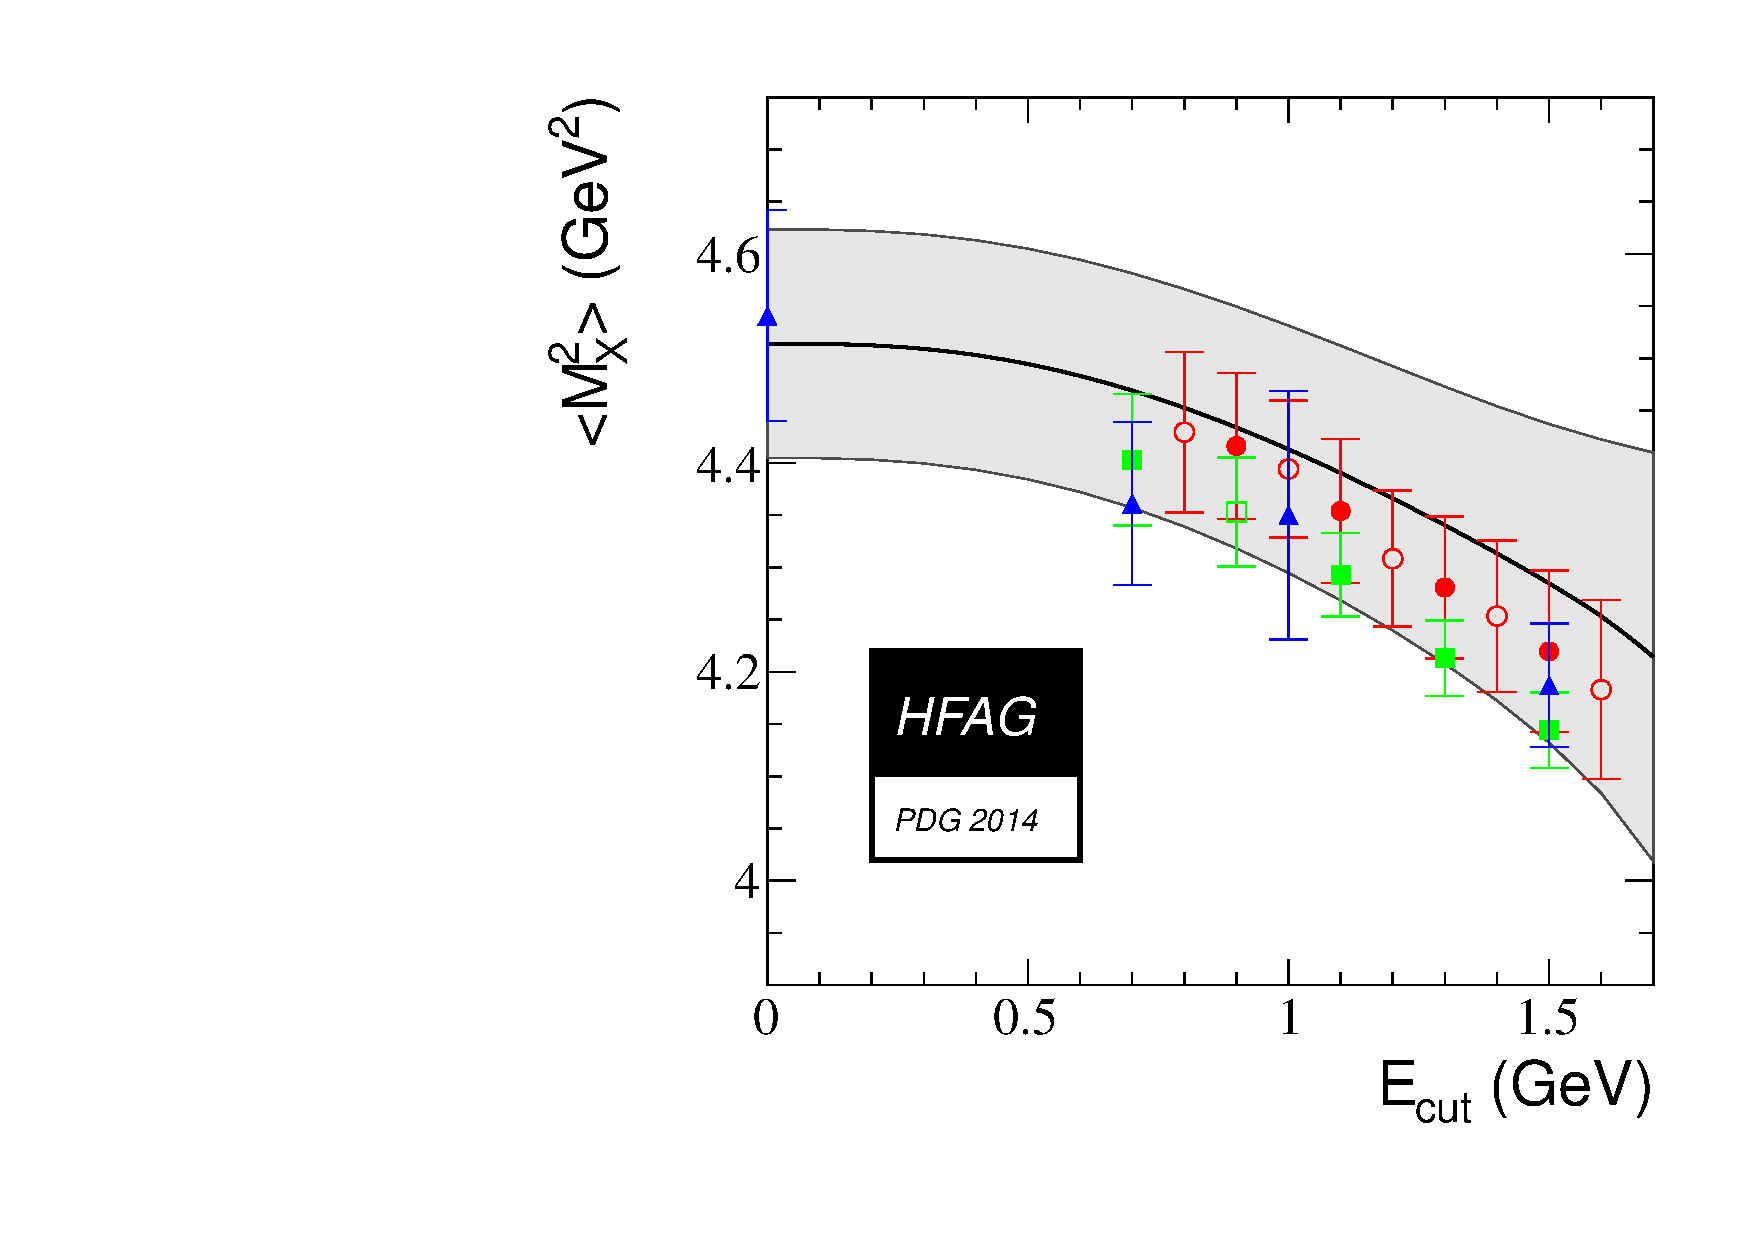
\includegraphics[width=7cm]{figures/slb/h1_1.pdf}
  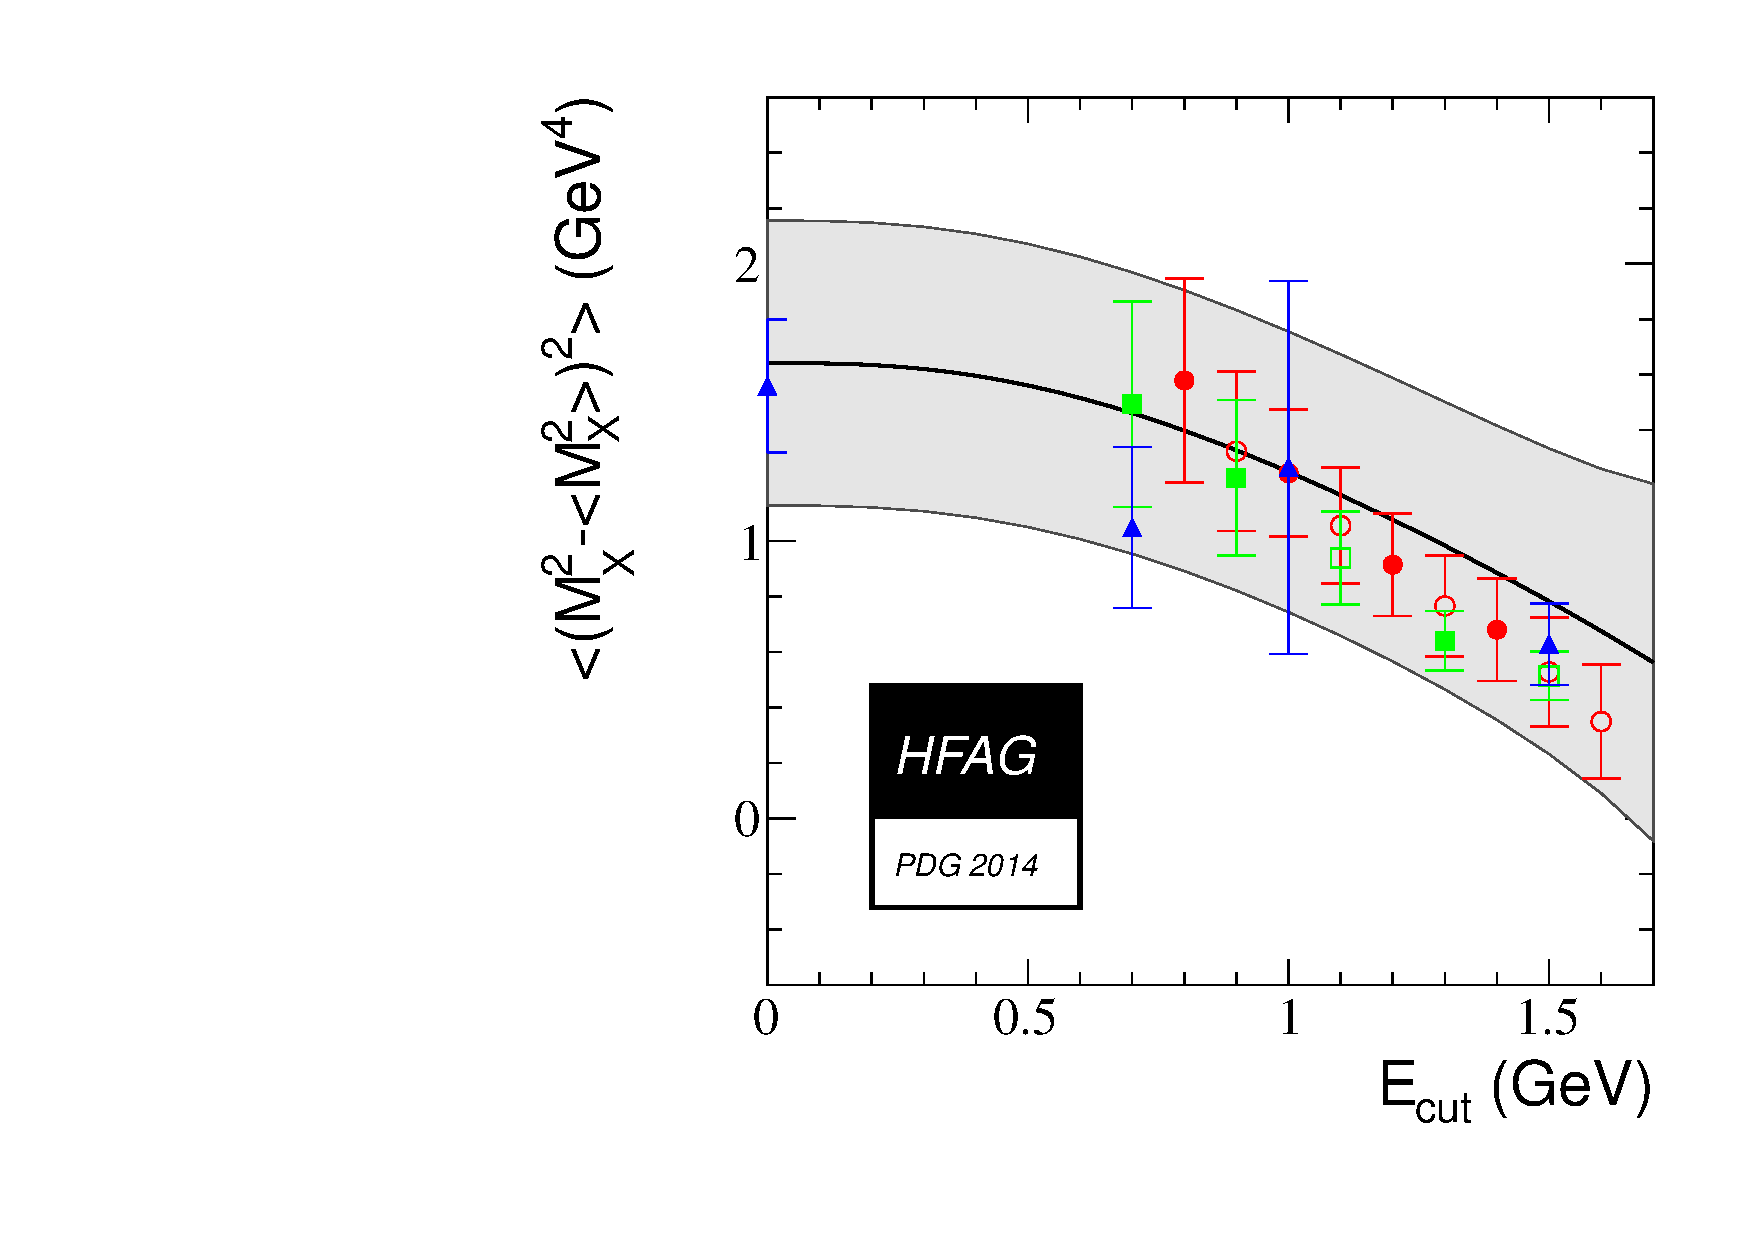
\includegraphics[width=7cm]{figures/slb/h2_1.pdf}\\
  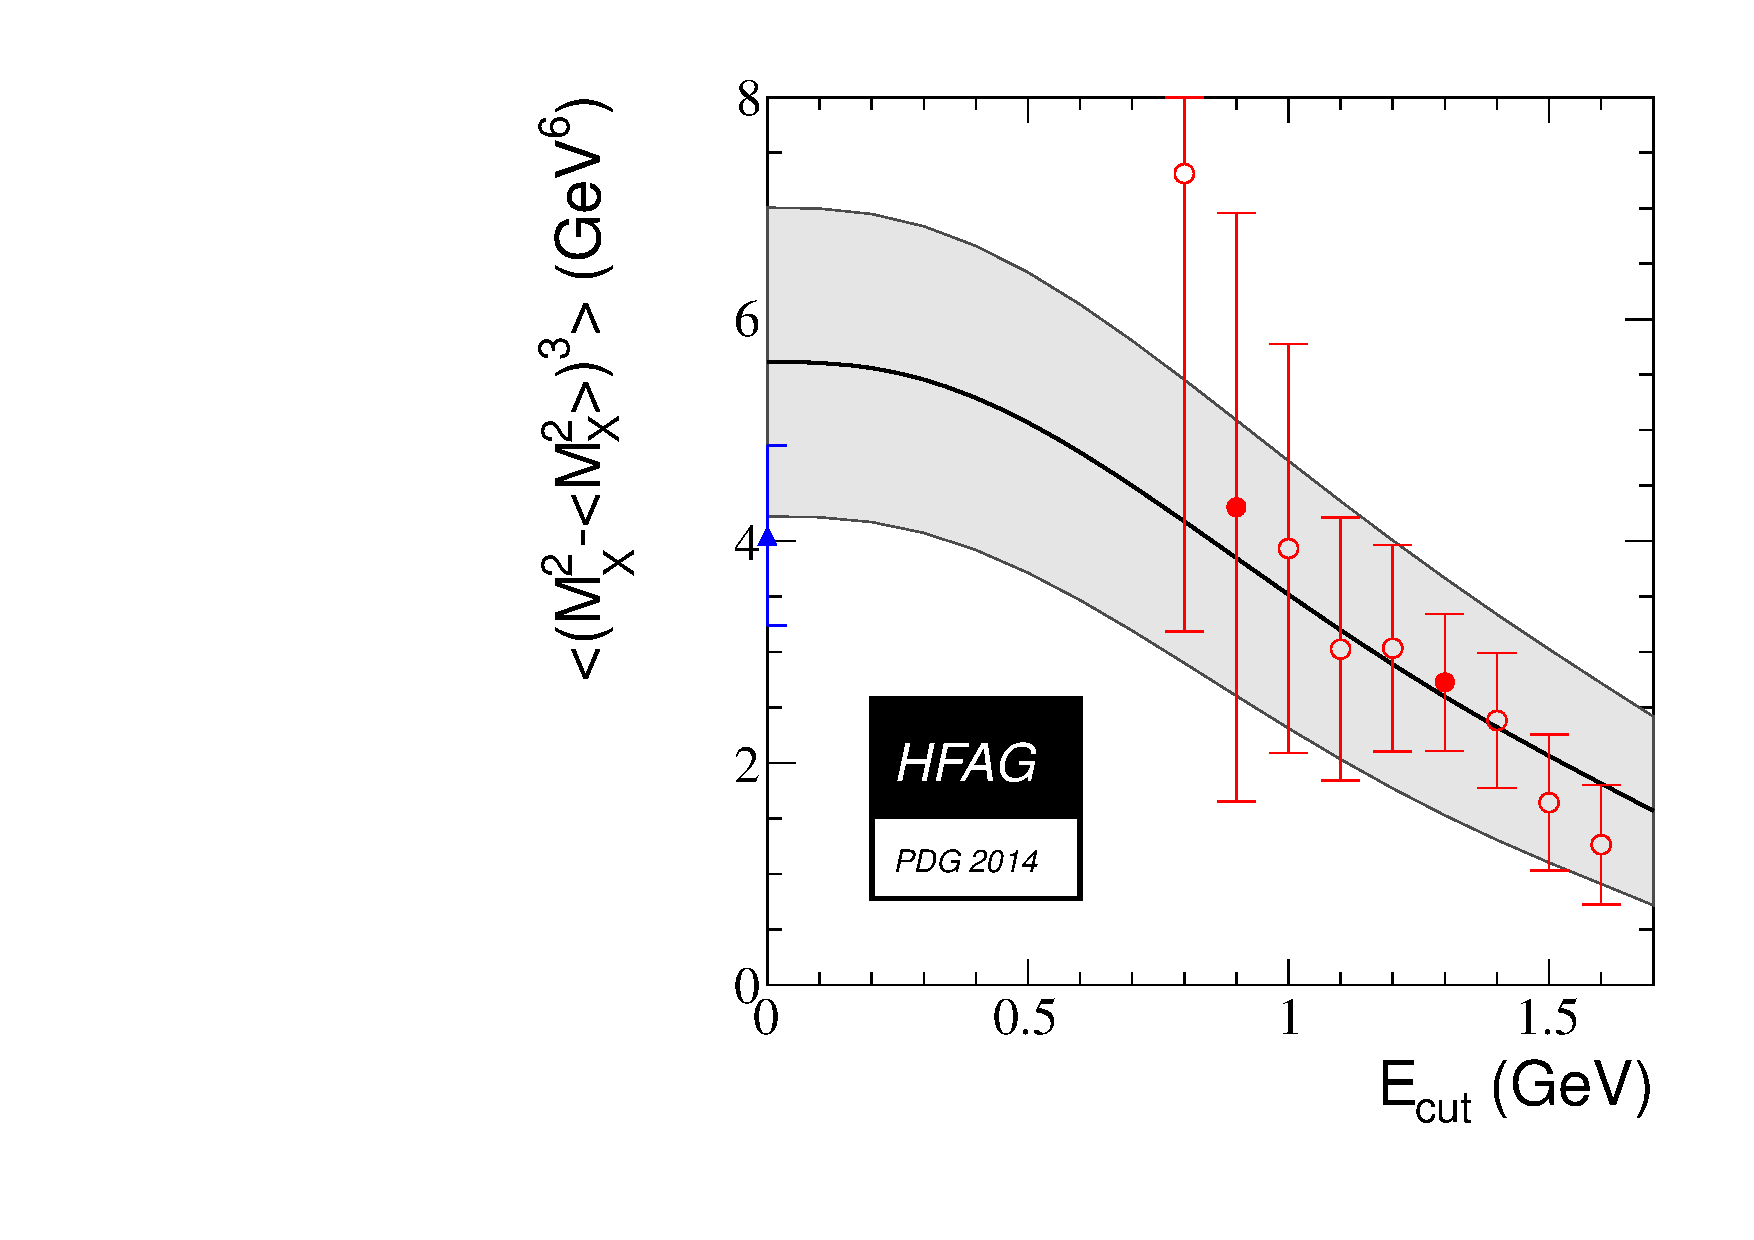
\includegraphics[width=7cm]{figures/slb/h3_1.pdf}
\end{center}
\caption{Same as Fig.~\ref{fig:gf_res_kin_el} for the fit to the
  hadronic mass moments in the kinetic mass
  scheme.} \label{fig:gf_res_kin_mx}
\end{figure}

The inclusive $\bar B\to X_c\ell^-\bar\nu_\ell$ branching fraction
determined by this analysis is
\begin{equation}
  \cbf(\bar B\to X_c\ell^-\bar\nu_\ell)=(10.65\pm 0.16)\%~.
\end{equation}
Correcting for charmless semileptonic decays
(Sect.~\ref{slbdecays_b2uincl}), $\cbf(\bar B\to
X_u\ell^-\bar\nu_\ell)=(2.14\pm 0.31)\times 10^{-3}$, we obtain the
semileptonic branching fraction,
\begin{equation}
  \cbf(\bar B\to X\ell^-\bar\nu_\ell)=(10.86\pm 0.16)\%~.
\end{equation}

\subsubsection{Analysis in the 1S scheme}
\label{globalfits1S}

The fit relies on the calculations of the spectral moments described in
Ref.~\cite{Bauer:2004ve}. The theoretical uncertainties are estimated
as explained in Ref.~\cite{Schwanda:2008kw}. Only trivial theory
correlations, {\it i.e.}, between the same moment at the same
threshold are included in the analysis. The fit determines $\vcb$ and
the 6 non-perturbative parameters mentioned above.

The result of the fit using the $B\to X_s\gamma$ constraint is
\begin{eqnarray}
  \vcb & = & (41.98\pm 0.45)\times 10^{-3}~, \\
  m_b^{1S} & = & 4.691\pm 0.037~{\rm GeV}~, \\
  \lambda_1 & = & -0.362\pm 0.067~{\rm GeV^2}~,
\end{eqnarray}
with a $\chi^2$ of 23.0 for $66-7$ degrees of freedom. The detailed
result of the fit is given in Table~\ref{tab:gf_res_xsgamma_1s}.
\begin{table}[!htb]
\caption{Fit result in the 1S scheme, using $B\to X_s\gamma$~moments
  as a constraint. In the lower part of the table, the correlation
  matrix of the parameters is given.} \label{tab:gf_res_xsgamma_1s}
\begin{center}
\begin{tabular}{|l|ccccccc|}
  \hline
  & $m_b^{1S}$ [GeV] & $\lambda_1$ [GeV$^2$] & $\rho_1$ [GeV$^3$] &
  $\tau_1$ [GeV$^3$] & $\tau_2$ [GeV$^3$] & $\tau_3$ [GeV$^3$] &
  $\vcb$ [10$^{-3}$]\\
  \hline \hline
  value & 4.691 & $-0.362$ & \phantom{$-$}0.043 &
  \phantom{$-$}0.161 & $-0.017$ & \phantom{$-$}0.213 &
  \phantom{$-$}41.98\\
  error & 0.037 & \phantom{$-$}0.067 & \phantom{$-$}0.048 &
  \phantom{$-$}0.122 & \phantom{$-$}0.062 & \phantom{$-$}0.102 &
  \phantom{$-$}0.45\\
  \hline
  $m_b^{1S}$ & 1.000 & \phantom{$-$}0.434 & \phantom{$-$}0.213 &
  $-0.058$ & $-0.629$ & $-0.019$ & $-0.215$\\
  $\lambda_1$ & & \phantom{$-$}1.000 & $-0.467$ & $-0.602$ & $-0.239$
  & $-0.547$ & $-0.403$\\
  $\rho_1$ & & & \phantom{$-$}1.000 & \phantom{$-$}0.129 & $-0.624$ &
  \phantom{$-$}0.494 & \phantom{$-$}0.286\\
  $\tau_1$ & & & & \phantom{$-$}1.000 & \phantom{$-$}0.062 & $-0.148$ &
  \phantom{$-$}0.194\\
  $\tau_2$ & & & & & \phantom{$-$}1.000 & $-0.009$ & $-0.145$\\
  $\tau_3$ & & & & & & \phantom{$-$}1.000 & \phantom{$-$}0.376\\
  $\vcb$ & & & & & & & \phantom{$-$}1.000\\
  \hline
\end{tabular}
\end{center}
\end{table}
